\chapter{Unit Tests}
% Beschreibung der Tests
Unit Tests haben die Aufgabe einzelne Einheiten von Code auf Funktionalität zu überprüfen. Dabei kann eine Einheit eine einzelne Methode, eine Klasse oder ein Modul sein. Zweck ist die Sicherstellung dass jede Einheit der Software wie erwartet funktioniert und dass Änderungen an einer Einheit keine unerwarteten Auswirkungen auf andere Teile der Software haben. Darüber hinaus helfen Unit-Tests auch dabei, die Qualität und Zuverlässigkeit der Software zu verbessern, da sie sicherstellen, dass jeder Teil des Codes wie erwartet funktioniert und dass Fehler vermieden werden. Unit-Tests tragen somit dazu bei, dass die Software insgesamt stabiler und robuster wird.
\section{10 Unit Tests}
%Nennung von 10 Unit-Tests und Beschreibung, was getestet wird
\begin{enumerate}
    \item UserBuildTest.testPerformActionBasedOnAnswers() Testet ob für jeden Simpsons Charakter eine Aktion bereitgestellt wird.
    \item ApuTest.testIntroduce() Testet ob die Methode introduce() den richtigen String zurückgibt. Die selben Tests wurden für die Simpsons Charaktere Bart, Homer, Marge, Lisa, Maggie, ComicBookGuy, Ned, Skinner und Nelson durchgeführt.
    \item SimpsonsCharacterTest.testFavoriteFood() Testet ob abhängig vom Charakter der Simpsons das spezifische Lieblingsessen zurückgegeben wird.
    \item SimpsonsCharacterTest.testPersonalTransport() Testet ob abhängig vom Charakter der Simpsons das spezifische Transportmittel zurückgegeben wird.
    \item ConsumerGoodsTest.testToString() Testet ob abhängig vom jeweiligen Enum der richtige String zum Lieblingsessen zurückgegeben wird.
    \item PersonalTransportTest.testDisplayName() Testet ob abhängig vom jeweiligen Enum der richtige String zum Transportmittel zurückgegeben wird.
    \item WorkplacesTest.testGettersAndSetters() Testet ob die Getter und Setter der Klasse Workplaces funktionieren.
\end{enumerate}

\section{ATRIP: Automatic}
%Begründung/Erläuterung, wie ‘Automatic’ realisiert wurde
Test sollten nach Möglichkeit automatisiert ablaufen. Des Weiteren sollten auch die Ergebnisse eines Tests auf ihren positiven oder negativen Ausgang geprüft werden. In diesem Projekt wird dies mit dem Surfire Plugin von Maven realisiert, welches, wie in Abbildung \ref{fig:surefire} zu sehen, alle Tests auf einmal abruft und angibt, ob ein Test fehlgeschlagen ist oder nicht. Abgerufen wird dieser Test mit dem Befehl 'mvn test' im Verzeichnis des Projekts über das Terminal.
\begin{figure}[ht]
    \centering
    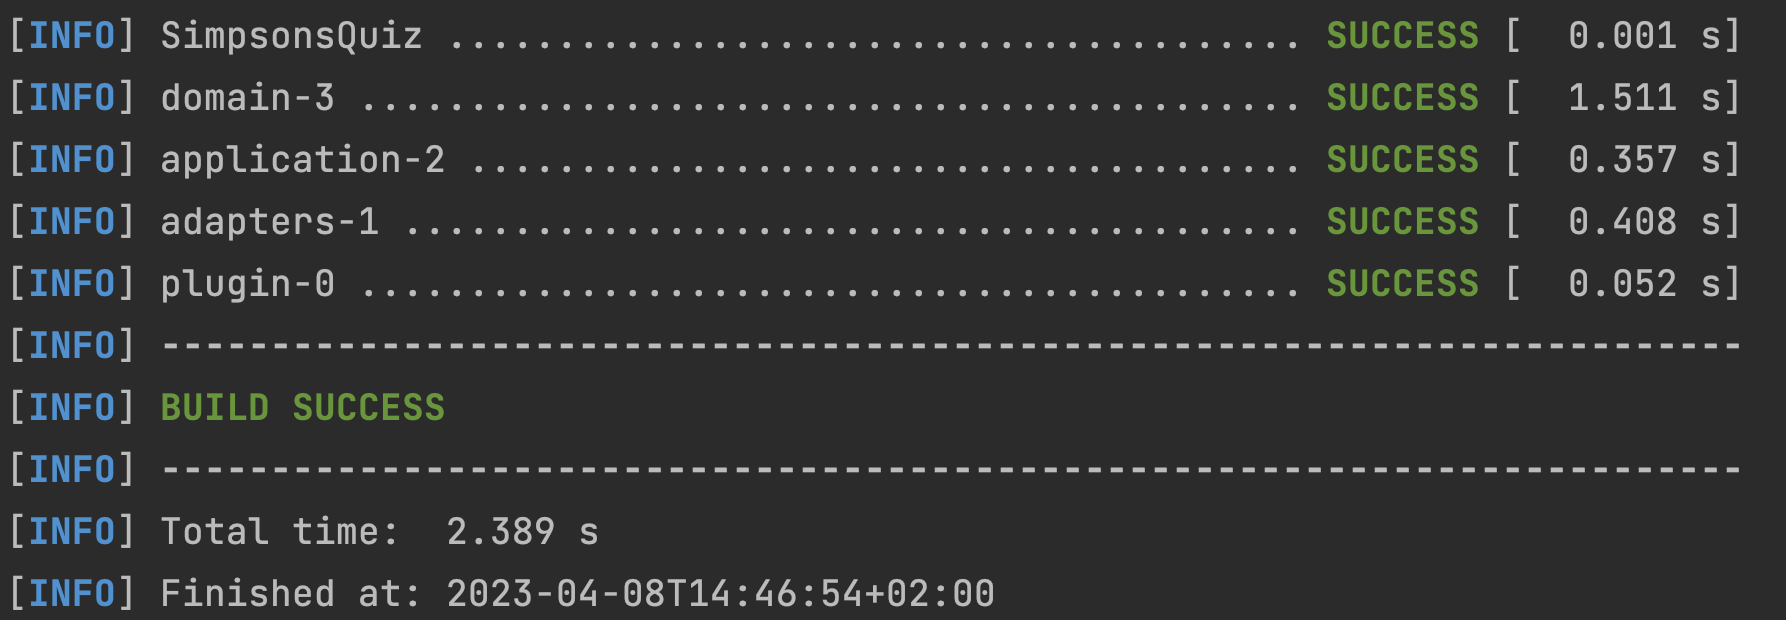
\includegraphics[width=0.8\textwidth]{Bilder/tests.png}
    \caption{Maven Surfire Plugin}
    \label{fig:surefire}
\end{figure}
\newpage

\section{ATRIP: Thorough}
% jeweils 1 positives und negatives Beispiel zu ‘Thorough’; jeweils Code-Beispiel, Analyse und Begründung, was gründlich/nicht gründlich ist
Thorough bezieht sich auf die Gründlichkeit eines Tests, insbesondere auf die vollständige Prüfung des gesamten Codes um sicherzustellen, dass alle Aspekte der Funktionalität geprüft und alle Szenarien abgedeckt wurden. In diesem Projekt wurde dies durch die Erstellung von Unit Tests für jeden einzelnen Simpsons Charakter sichergestellt, wie in listing \ref{code:apuTest} zu sehen ist. Die Tests prüfen, ob die Methode introduce() den richtigen String zurückgibt. Die selben Tests wurden für die Simpsons Charaktere Bart, Homer, Marge, Lisa, Maggie, ComicBookGuy, Ned, Skinner und Nelson durchgeführt.

\lstinputlisting[
	label=code:apuTest,    % Label; genutzt für Referenzen auf dieses Code-Beispiel
	caption=Unit Test der Klasse Apu,
	captionpos=b,               % Position, an der die Caption angezeigt wird t(op) oder b(ottom)
	style=EigenerJavaStyle,     % Eigener Style der vor dem Dokument festgelegt wurde
	firstline=1,                % Zeilennummer im Dokument welche als erste angezeigt wird
	lastline=12                 % Letzte Zeile welche ins LaTeX Dokument übernommen wird
]{Quellcode/apu.java}
Negativ gilt an dieser Stelle hervorzuheben, dass nicht alle Methoden der jeweiligen Klassen getestet werden. Nur wenn alle Methoden vollständig durch Unit Tests abgedeckt sind, gilt das Prinzip erfüllt.  
\section{ATRIP: Professional}
% jeweils 1 positives und negatives Beispiel zu ‘Professional’; jeweils Code-Beispiel, Analyse und Begründung, was professionell/nicht professionell ist
Da Tests den selben Qualitätsstandards wie Produktivcode unterliegen, sollte auch hierbei darauf geachtet werden, dass die Tests mit der notwendigen Professionalität erstellt werden. Dies bedeutet, dass die Tests gut lesbar und wartbar sind. Außerdem sollten sie so geschrieben werden, dass sie leicht zu verstehen sind und dass sie sich leicht erweitern lassen. Ein positives Beispiel ist die der Test des User Builds in listing \ref{code:userBuildTest}. Dieser Test prüft, ob für jeden Simpsons Charakter eine Aktion bereitgestellt wird. Dies wird durch die Methode testPerformActionBasedOnAnswers() realisiert. Dabei spielt es keine Rolle wie viele Charakter momentan vorhanden sind, oder ob noch welche hinzugefügt werden. 
\lstinputlisting[
    label=code:userBuildTest,    % Label; genutzt für Referenzen auf dieses Code-Beispiel
    caption=Unit Test der Klasse UserBuild,
    captionpos=b,               % Position, an der die Caption angezeigt wird t(op) oder b(ottom)
    style=EigenerJavaStyle,     % Eigender Style der vor dem Dokument festgelegt wurde
    firstline=1,                % Zeilennummer im Dokument welche als erste angezeigt wird
    lastline=9                 % Letzte Zeile welche ins LaTeX Dokument übernommen wird
]{Quellcode/goodtest.java} 
\newpage

Unnötige Tests wie beispielsweise der Test von Getter und Setter Methoden sind hingegen nicht professionell. Dies ist in listing \ref{code:badtest} zu sehen. Dieser Test prüft, ob die Getter und Setter der Klasse Workplaces funktionieren. Dies ist unnötig, da man keine Tests nur des Testens wegen schreiben sollte.
\lstinputlisting[
    label=code:badtest,    % Label; genutzt für Referenzen auf dieses Code-Beispiel
    caption=Unit Test der Klasse Workplaces,
    captionpos=b,               % Position, an der die Caption angezeigt wird t(op) oder b(ottom)
    style=EigenerJavaStyle,     % Eigender Style der vor dem Dokument festgelegt wurde
    firstline=1,                % Zeilennummer im Dokument welche als erste angezeigt wird
    lastline=23                 % Letzte Zeile welche ins LaTeX Dokument übernommen wird
]{Quellcode/badtest.java}
\newpage

\section{Code Coverage}
% Code Coverage im Projekt analysieren und begründen
Code Coverage ist ein Maß dafür, wie viel Prozent des Quellcodes einer Software durch Tests abgedeckt werden. Eine Code Coverage von 100\% würde bedeuten, dass jeder Teil des Codes durch Tests abgedeckt wurde, während eine  niedrigere Code Coverage darauf hinweist, dass einige Teile des Codes nicht durch Tests überprüft wurden. In diesem Projekt wurde die Code Coverage mit dem JaCoCo Plugin von Maven ermittelt. Dieses Plugin ist in Abbildung \ref{fig:jacoco} zu sehen. Die Code Coverage beträgt 24\% der Klassen und 17\% der Methoden, womit also noch Bedarf an Optimierung besteht.
\begin{figure}[ht]
    \centering
    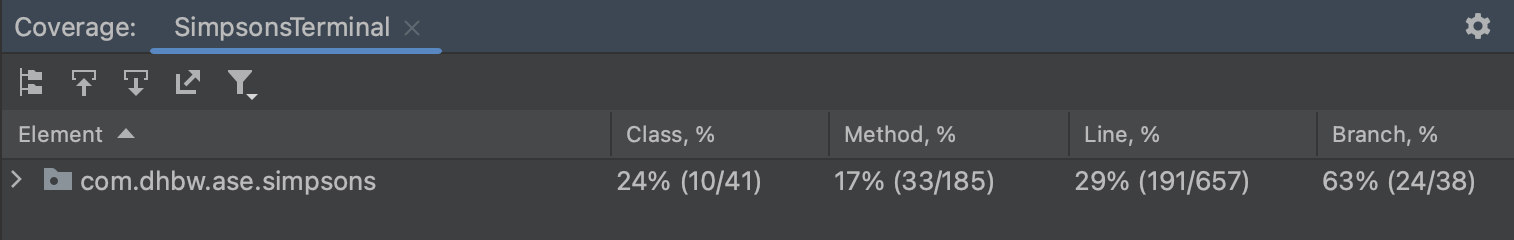
\includegraphics[width=0.8\textwidth]{Bilder/coverage.png}
    \caption{Maven JaCoCo Plugin}
    \label{fig:jacoco}
\end{figure}
\newpage

\section{Fakes und Mocks}
% Analyse und Begründung des Einsatzes von 2 Fake/Mock-Objekten; zusätzlich jeweils UML Diagramm der Klasse
Mocks sind im Kontext von Unit-Tests Platzhalter-Objekte, die das Verhalten von Abhängigkeiten simulieren, die für den Test nicht verfügbar sind oder unerwünschte Nebenwirkungen haben könnten. Sie helfen, Tests schneller auszuführen, indem sie die Interaktionen der zu testenden Komponente mit ihren Abhängigkeiten imitieren. Mocks können auch zur Überprüfung von Interaktionen verwendet werden, indem sie aufgezeichnete Methodenaufrufe und Parameter speichern und anschließend überprüfen, ob sie den erwarteten Werten entsprechen. In diesem Projekt wird, wie in listing \ref{code:mock} zu sehen, der Unit Test QuestionManagerTest als Mock Klasse verwendet um die Eingabe durch einen Nutzer zu simulieren. 
\lstinputlisting[
    label=code:mock,    % Label; genutzt für Referenzen auf dieses Code-Beispiel
    caption=Mock Klasse für den Question Manager,
    captionpos=b,               % Position, an der die Caption angezeigt wird t(op) oder b(ottom)
    style=EigenerJavaStyle,     % Eigender Style der vor dem Dokument festgelegt wurde
    firstline=1,                % Zeilennummer im Dokument welche als erste angezeigt wird
    lastline=33                 % Letzte Zeile welche ins LaTeX Dokument übernommen wird
]{Quellcode/mock.java}

Die Mock-Klasse enthält eine Test-Methode testAskQuestions (), die eine Instanz von QuestionManager erstellt und die askQuestions() - Methode dieser Instanz testet. Zunächst wird eine zufällige Benutzereingabe erstellt, indem eine StringBuilder-Instanz mit der Größe der charToName-Map der QuestionManager-Klasse initialisiert wird. Die Schleife durchläuft dann jede Zeichenposition und fügt zufällig 'y' für Ja oder 'n' für Nein hinzu, um die Benutzereingabe zu simulieren. Anschließend wird eine InputStream-Instanz erstellt, um die generierte Benutzereingabe zu setzen. Dann wird die askQuestions () -Methode aufgerufen, um die Antwort des Frage-Managers zu erhalten. Schließlich wird geprüft, ob das Ergebnis ein gültiges Zeichen enthält, das in der Liste der erwarteten Zeichen "validChars" enthalten ist.